% Options for packages loaded elsewhere
% Options for packages loaded elsewhere
\PassOptionsToPackage{unicode}{hyperref}
\PassOptionsToPackage{hyphens}{url}
\PassOptionsToPackage{dvipsnames,svgnames,x11names}{xcolor}
%
\documentclass[
  french,
  10pt,
  a4paper,
]{scrartcl}
\usepackage{xcolor}
\usepackage[top=1.7cm,bottom=1.7cm,left=1.6cm,right=1.6cm,headsep=0.35cm,footskip=0.75cm,includeheadfoot]{geometry}
\usepackage{amsmath,amssymb}
\setcounter{secnumdepth}{-\maxdimen} % remove section numbering
\usepackage{iftex}
\ifPDFTeX
  \usepackage[T1]{fontenc}
  \usepackage[utf8]{inputenc}
  \usepackage{textcomp} % provide euro and other symbols
\else % if luatex or xetex
  \usepackage{unicode-math} % this also loads fontspec
  \defaultfontfeatures{Scale=MatchLowercase}
  \defaultfontfeatures[\rmfamily]{Ligatures=TeX,Scale=1}
\fi
\usepackage{lmodern}
\ifPDFTeX\else
  % xetex/luatex font selection
\fi
% Use upquote if available, for straight quotes in verbatim environments
\IfFileExists{upquote.sty}{\usepackage{upquote}}{}
\IfFileExists{microtype.sty}{% use microtype if available
  \usepackage[]{microtype}
  \UseMicrotypeSet[protrusion]{basicmath} % disable protrusion for tt fonts
}{}
\makeatletter
\@ifundefined{KOMAClassName}{% if non-KOMA class
  \IfFileExists{parskip.sty}{%
    \usepackage{parskip}
  }{% else
    \setlength{\parindent}{0pt}
    \setlength{\parskip}{6pt plus 2pt minus 1pt}}
}{% if KOMA class
  \KOMAoptions{parskip=half}}
\makeatother
% Make \paragraph and \subparagraph free-standing
\makeatletter
\ifx\paragraph\undefined\else
  \let\oldparagraph\paragraph
  \renewcommand{\paragraph}{
    \@ifstar
      \xxxParagraphStar
      \xxxParagraphNoStar
  }
  \newcommand{\xxxParagraphStar}[1]{\oldparagraph*{#1}\mbox{}}
  \newcommand{\xxxParagraphNoStar}[1]{\oldparagraph{#1}\mbox{}}
\fi
\ifx\subparagraph\undefined\else
  \let\oldsubparagraph\subparagraph
  \renewcommand{\subparagraph}{
    \@ifstar
      \xxxSubParagraphStar
      \xxxSubParagraphNoStar
  }
  \newcommand{\xxxSubParagraphStar}[1]{\oldsubparagraph*{#1}\mbox{}}
  \newcommand{\xxxSubParagraphNoStar}[1]{\oldsubparagraph{#1}\mbox{}}
\fi
\makeatother


\usepackage{longtable,booktabs,array}
\newcounter{none} % for unnumbered tables
\usepackage{calc} % for calculating minipage widths
% Correct order of tables after \paragraph or \subparagraph
\usepackage{etoolbox}
\makeatletter
\patchcmd\longtable{\par}{\if@noskipsec\mbox{}\fi\par}{}{}
\makeatother
% Allow footnotes in longtable head/foot
\IfFileExists{footnotehyper.sty}{\usepackage{footnotehyper}}{\usepackage{footnote}}
\makesavenoteenv{longtable}
\usepackage{graphicx}
\makeatletter
\newsavebox\pandoc@box
\newcommand*\pandocbounded[1]{% scales image to fit in text height/width
  \sbox\pandoc@box{#1}%
  \Gscale@div\@tempa{\textheight}{\dimexpr\ht\pandoc@box+\dp\pandoc@box\relax}%
  \Gscale@div\@tempb{\linewidth}{\wd\pandoc@box}%
  \ifdim\@tempb\p@<\@tempa\p@\let\@tempa\@tempb\fi% select the smaller of both
  \ifdim\@tempa\p@<\p@\scalebox{\@tempa}{\usebox\pandoc@box}%
  \else\usebox{\pandoc@box}%
  \fi%
}
% Set default figure placement to htbp
\def\fps@figure{htbp}
\makeatother



\ifLuaTeX
\usepackage[bidi=basic,shorthands=off]{babel}
\else
\usepackage[bidi=default,shorthands=off]{babel}
\fi
\ifLuaTeX
  \usepackage{selnolig} % disable illegal ligatures
\fi


\setlength{\emergencystretch}{3em} % prevent overfull lines

\providecommand{\tightlist}{%
  \setlength{\itemsep}{0pt}\setlength{\parskip}{0pt}}



 


% Mise en page des PDF : LaTeX classique (Latin Modern), A4, compacte,
% entièrement lisible en noir et blanc. Chargé après le préambule de Quarto.
\usepackage{xcolor}
\definecolor{vertprofond}{HTML}{1C322D}
\definecolor{grisfilet}{HTML}{A1A1AA}

% Paragraphes sans alinéa, séparés par un petit espace.
\setlength{\parindent}{0pt}
\setlength{\parskip}{0.5ex plus 0.2ex minus 0.1ex}

% Titres resserrés, en vert profond (assez sombre pour l'impression N&B).
\setkomafont{disposition}{\normalfont\bfseries\color{vertprofond}}
\setkomafont{section}{\large}
\setkomafont{subsection}{\normalsize}
\setkomafont{subsubsection}{\normalsize\itshape}
\RedeclareSectionCommand[beforeskip=-1.6ex plus -0.4ex minus -0.2ex,
  afterskip=0.6ex plus 0.1ex]{section}
\RedeclareSectionCommand[beforeskip=-1.2ex plus -0.3ex minus -0.2ex,
  afterskip=0.4ex plus 0.1ex]{subsection}
\RedeclareSectionCommand[beforeskip=-1ex plus -0.2ex,
  afterskip=0.3ex]{subsubsection}

% Listes serrées.
\usepackage{enumitem}
\setlist{topsep=0.3ex, itemsep=0.15ex, parsep=0pt, partopsep=0pt}

% Figures et tableaux : peu d'espace autour, images plafonnées en hauteur
% pour qu'un schéma n'occupe jamais une demi-page.
\setlength{\textfloatsep}{1.2ex plus 0.4ex minus 0.4ex}
\setlength{\floatsep}{1ex plus 0.4ex minus 0.4ex}
\setlength{\intextsep}{1ex plus 0.4ex minus 0.4ex}
\setlength{\abovecaptionskip}{0.4ex}
\setlength{\belowcaptionskip}{0pt}
\setkomafont{caption}{\small\itshape}
\setkomafont{captionlabel}{\small\itshape}
\setkeys{Gin}{width=\linewidth, height=0.28\textheight, keepaspectratio}
\renewcommand{\arraystretch}{1.15}

% En-tête et pied de page : formation et chapitre en haut, titre et
% numéro de page en bas. Les valeurs viennent du partial title.tex.
\usepackage{lastpage}
\usepackage[headsepline=0.4pt, footsepline=0.4pt]{scrlayer-scrpage}
\clearpairofpagestyles
\setkomafont{pageheadfoot}{\footnotesize\color{vertprofond}}
\setkomafont{pagenumber}{}
\ihead{\vintageformation}
\ohead{\vintagechapitre}
\ifoot*{\vintagetitre}
\ofoot*{\thepage\,/\,\pageref*{LastPage}}
\pagestyle{scrheadings}

% Schémas TikZ : les styles communs suivent dans tikz-vintage.tex.
\usepackage{tikz}
% Styles TikZ communs aux schémas du site (PDF et HTML).
% Lisibles en noir et blanc : le contraste vient des niveaux de gris,
% des traits (plein, tirets, pointillés) et des étiquettes, jamais de la
% seule couleur. Le vert profond de la charte sert de couleur d'encre.
\usetikzlibrary{arrows.meta, positioning, calc, fit, backgrounds,
  shapes.geometric, shapes.symbols, patterns, decorations.pathreplacing}
\definecolor{vertprofond}{HTML}{1C322D}
\definecolor{grisclair}{HTML}{E4E4E7}
\definecolor{grismoyen}{HTML}{A1A1AA}
\tikzset{
  >={Stealth[length=2.2mm]},
  every picture/.style={color=vertprofond, line width=0.6pt},
  every node/.style={font=\small},
  % Équipements
  poste/.style={draw, rounded corners=1.5pt, fill=white,
    minimum width=1.4cm, minimum height=0.8cm, align=center},
  serveur/.style={poste, fill=grisclair, minimum height=1cm},
  routeur/.style={draw, circle, fill=grisclair, minimum size=1cm,
    align=center, font=\small\bfseries},
  commutateur/.style={draw, fill=grismoyen!40, minimum width=2.4cm,
    minimum height=0.6cm, align=center, font=\small\bfseries},
  parefeu/.style={draw, fill=white,
    postaction={pattern=bricks, pattern color=grismoyen},
    minimum width=1.2cm, minimum height=0.9cm, font=\small\bfseries},
  nuage/.style={draw, cloud, cloud puffs=10, aspect=2, fill=white,
    align=center},
  % Liaisons
  lien/.style={line width=0.9pt},
  trunk/.style={line width=2pt},
  sans fil/.style={dashed},
  % Échanges de messages (diagrammes de séquence)
  ligne de vie/.style={dashed, grismoyen},
  message/.style={->},
  diffusion/.style={->, dashed},
  reponse/.style={->, densely dotted},
  % Annotations
  etiquette/.style={font=\footnotesize, inner sep=1pt, fill=white},
  adresse/.style={font=\footnotesize\ttfamily, inner sep=1pt},
  zone/.style={draw, dashed, rounded corners=4pt, inner sep=6pt},
}
\makeatletter
\@ifpackageloaded{tcolorbox}{}{\usepackage[skins,breakable]{tcolorbox}}
\@ifpackageloaded{fontawesome5}{}{\usepackage{fontawesome5}}
\definecolor{quarto-callout-color}{HTML}{909090}
\definecolor{quarto-callout-note-color}{HTML}{0758E5}
\definecolor{quarto-callout-important-color}{HTML}{CC1914}
\definecolor{quarto-callout-warning-color}{HTML}{EB9113}
\definecolor{quarto-callout-tip-color}{HTML}{00A047}
\definecolor{quarto-callout-caution-color}{HTML}{FC5300}
\definecolor{quarto-callout-color-frame}{HTML}{acacac}
\definecolor{quarto-callout-note-color-frame}{HTML}{4582ec}
\definecolor{quarto-callout-important-color-frame}{HTML}{d9534f}
\definecolor{quarto-callout-warning-color-frame}{HTML}{f0ad4e}
\definecolor{quarto-callout-tip-color-frame}{HTML}{02b875}
\definecolor{quarto-callout-caution-color-frame}{HTML}{fd7e14}
\makeatother
\makeatletter
\@ifpackageloaded{caption}{}{\usepackage{caption}}
\AtBeginDocument{%
\ifdefined\contentsname
  \renewcommand*\contentsname{Table des matières}
\else
  \newcommand\contentsname{Table des matières}
\fi
\ifdefined\listfigurename
  \renewcommand*\listfigurename{Liste des Figures}
\else
  \newcommand\listfigurename{Liste des Figures}
\fi
\ifdefined\listtablename
  \renewcommand*\listtablename{Liste des Tables}
\else
  \newcommand\listtablename{Liste des Tables}
\fi
\ifdefined\figurename
  \renewcommand*\figurename{Figure}
\else
  \newcommand\figurename{Figure}
\fi
\ifdefined\tablename
  \renewcommand*\tablename{Table}
\else
  \newcommand\tablename{Table}
\fi
}
\@ifpackageloaded{float}{}{\usepackage{float}}
\floatstyle{ruled}
\@ifundefined{c@chapter}{\newfloat{codelisting}{h}{lop}}{\newfloat{codelisting}{h}{lop}[chapter]}
\floatname{codelisting}{Listing}
\newcommand*\listoflistings{\listof{codelisting}{Liste des Listings}}
\makeatother
\makeatletter
\makeatother
\makeatletter
\@ifpackageloaded{caption}{}{\usepackage{caption}}
\@ifpackageloaded{subcaption}{}{\usepackage{subcaption}}
\makeatother
\usepackage{bookmark}
\IfFileExists{xurl.sty}{\usepackage{xurl}}{} % add URL line breaks if available
\urlstyle{same}
% fallback for those not using the hyperref driver hyperxmp:
\makeatletter
\@ifundefined{xmpquote}{\newcommand{\xmpquote}[1]{#1}}{}
\makeatother
\hypersetup{
  pdftitle={TP2 (partie 3) --- Réseau sans fil et cahier des charges},
  pdflang={fr},
  colorlinks=true,
  linkcolor={vertprofond},
  filecolor={Maroon},
  citecolor={Blue},
  urlcolor={vertprofond},
  pdfcreator={LaTeX via pandoc}}


\newcommand{\vintagetitre}{TP2 (partie 3) --- Réseau sans fil et cahier
des charges}
\newcommand{\vintageformation}{BTS CIEL 1}
\newcommand{\vintagechapitre}{01 --- Introduction aux réseaux}
\title{TP2 (partie 3) --- Réseau sans fil et cahier des charges}
\author{}
\date{}
\begin{document}
\thispagestyle{plain.scrheadings}
{\footnotesize\color{vertprofond}\textsc{BTS CIEL 1}\enspace·\enspace 01
--- Introduction aux réseaux\hfill \textsc{tp}\enspace·\enspace 2 h\par}
\vspace{0.6ex}
{\LARGE\bfseries\color{vertprofond}TP2 (partie 3) --- Réseau sans fil et
cahier des charges\par}
\vspace{0.5ex}
{\itshape Construire un réseau Wi-Fi sécurisé dans Packet Tracer,
observer l'adressage dynamique, puis concevoir trois réseaux qui
répondent à un cahier des charges et les interconnecter.\par}
\vspace{0.3ex}
{\color{vertprofond}\rule{\linewidth}{0.8pt}\par}
\vspace{0.8ex}


\emph{Plateforme : Cisco Packet Tracer.}

\subsection{Objectifs et prérequis}\label{objectifs-et-pruxe9requis}

Votre téléphone se connecte à la box sans aucun câble. Dans ce TP, vous
reproduisez cette situation dans Packet Tracer. Vous terminez ensuite le
TP2 par un projet : trois réseaux à construire et à relier.

Dans cette dernière partie du TP2, vous allez :

\begin{itemize}
\tightlist
\item
  simuler un réseau sans fil (Wi-Fi) ;
\item
  comprendre pourquoi un appareil reçoit parfois une adresse inattendue
  ;
\item
  créer des réseaux qui répondent à un cahier des charges ;
\item
  configurer des réseaux différents pour qu'ils communiquent entre eux ;
\item
  calculer l'adresse réseau et l'adresse de diffusion d'un réseau.
\end{itemize}

Vous avez réalisé les parties 1 et 2 du TP2 : vous savez créer un
réseau, adresser des postes, utiliser un commutateur et un routeur.
Reprenez au besoin la \href{../tp-creation-lan-2/index.qmd}{partie 2} et
le \href{../tp-reseau-domestique/index.qmd}{TP1 --- Réseau domestique}.

\begin{tcolorbox}[enhanced jigsaw, arc=.35mm, bottomrule=.15mm, bottomtitle=1mm, breakable, colback=white, colbacktitle=quarto-callout-tip-color!10!white, colframe=quarto-callout-tip-color-frame, coltitle=black, left=2mm, leftrule=.75mm, opacityback=0, opacitybacktitle=0.6, rightrule=.15mm, title=\textcolor{quarto-callout-tip-color}{\faLightbulb}\hspace{0.5em}{Support d'activité}, titlerule=0mm, toprule=.15mm, toptitle=1mm]

\begin{itemize}
\tightlist
\item
  Cisco Packet Tracer, suite bureautique
\item
  Internet
\end{itemize}

\end{tcolorbox}

Vous rédigerez un compte rendu numérique. Pensez aux captures d'écran
pour illustrer votre compte rendu. Sauvegardez votre travail
régulièrement ! Des différences peuvent exister selon la version du
logiciel utilisée.

\subsection{Situation de départ}\label{situation-de-duxe9part}

Vous avez relié des postes avec des câbles, des concentrateurs, un
commutateur et un routeur. Il reste deux défis. Le premier est de se
passer de câbles : c'est le rôle du point d'accès Wi-Fi. Le second est
de concevoir vous-même des réseaux à partir d'un cahier des charges,
sans schéma de câblage fourni.

Résultat attendu en fin de séance :

\begin{itemize}
\tightlist
\item
  un réseau Wi-Fi sécurisé où un serveur, un ordinateur portable, une
  tablette et un smartphone communiquent ;
\item
  trois réseaux construits selon leur cahier des charges, puis reliés
  par un seul routeur ;
\item
  les adresses réseau et de diffusion du réseau 1, calculées.
\end{itemize}

\subsection{Matériel et
environnement}\label{matuxe9riel-et-environnement}

\begin{itemize}
\tightlist
\item
  Cisco Packet Tracer, sur votre poste.
\item
  Un nouveau fichier pour la partie A, puis un autre pour la partie B.
  Enregistrez-les sous des noms distincts.
\end{itemize}

\begin{longtable}[]{@{}lll@{}}
\caption{Déroulement de la séance}\label{tbl-deroulement}\tabularnewline
\toprule\noalign{}
Partie & Contenu & Durée indicative \\
\midrule\noalign{}
\endfirsthead
\toprule\noalign{}
Partie & Contenu & Durée indicative \\
\midrule\noalign{}
\endhead
\bottomrule\noalign{}
\endlastfoot
A & Créer un réseau sans fil (Wi-Fi) & 1 h \\
B & Créer trois réseaux et les relier & 1 h \\
\end{longtable}

\subsection{Travail à réaliser}\label{travail-uxe0-ruxe9aliser}

\subsubsection{Partie A --- Création d'un réseau sans fil (Wi-Fi) (1
h)}\label{partie-a-cruxe9ation-dun-ruxe9seau-sans-fil-wi-fi-1-h}

\begin{tcolorbox}[enhanced jigsaw, arc=.35mm, bottomrule=.15mm, bottomtitle=1mm, breakable, colback=white, colbacktitle=quarto-callout-note-color!10!white, colframe=quarto-callout-note-color-frame, coltitle=black, left=2mm, leftrule=.75mm, opacityback=0, opacitybacktitle=0.6, rightrule=.15mm, title=\textcolor{quarto-callout-note-color}{\faInfo}\hspace{0.5em}{Question 1}, titlerule=0mm, toprule=.15mm, toptitle=1mm]

Créez un nouveau fichier, construisez le réseau conformément au schéma
ci-dessous.

\end{tcolorbox}

\begin{figure}[htbp]

{\centering \pandocbounded{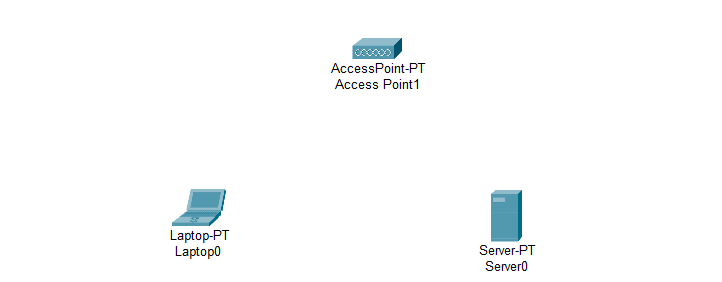
\includegraphics[keepaspectratio,alt={Capture d\textquotesingle écran de Packet Tracer : un point d\textquotesingle accès nommé Access Point1, de modèle AccessPoint-PT, est placé en haut. En bas, un ordinateur portable Laptop0 est à gauche et un serveur Server0 est à droite. Aucun lien ne relie encore les trois appareils.}]{img/schema-wifi-depart.png}}

}

\caption{Point d'accès, ordinateur portable et serveur : le réseau de
départ.}

\end{figure}%

\paragraph{Installer les modules
Wi-Fi}\label{installer-les-modules-wi-fi}

Un ordinateur ou un serveur de Packet Tracer est livré avec une carte
réseau filaire. Pour qu'il se connecte au point d'accès, il faut la
remplacer par un module sans fil.

\textbf{Pour le serveur} : cliquez sur le serveur pour ouvrir sa fenêtre
de propriétés, onglet « Physical ». Sur la face arrière visible,
éteignez le serveur. Remplacez le connecteur FastEthernet
(PT-HOST-MM-1CFE) par un connecteur wireless (PT-HOST-NM-1W). Rallumez
le serveur.

\textbf{Pour l'ordinateur portable} : cliquez sur le laptop pour ouvrir
sa fenêtre de propriétés, onglet « Physical ». Éteignez l'ordinateur
portable et ajoutez un module Wi-Fi tel que le WPC300N ou
PT-LAPTOP-NM-1W dans un slot libre. Rallumez l'ordinateur portable.

\begin{tcolorbox}[enhanced jigsaw, arc=.35mm, bottomrule=.15mm, bottomtitle=1mm, breakable, colback=white, colbacktitle=quarto-callout-important-color!10!white, colframe=quarto-callout-important-color-frame, coltitle=black, left=2mm, leftrule=.75mm, opacityback=0, opacitybacktitle=0.6, rightrule=.15mm, title=\textcolor{quarto-callout-important-color}{\faExclamation}\hspace{0.5em}{Choisir le bon module}, titlerule=0mm, toprule=.15mm, toptitle=1mm]

Assurez-vous d'utiliser les modules appropriés selon le type d'appareil
:

\begin{itemize}
\tightlist
\item
  WPC300N ou PT-LAPTOP-NM-1W pour les ordinateurs portables ;
\item
  PT-HOST-NM-1W pour les serveurs et les PC de bureau.
\end{itemize}

\end{tcolorbox}

Une fois les modules Wi-Fi installés sur tous les appareils, ils
pourront détecter et se connecter au réseau sans fil du point d'accès.

\paragraph{Adresser les appareils}\label{adresser-les-appareils}

Vous allez maintenant donner au serveur une adresse IP statique et un
masque de sous-réseau :

\begin{itemize}
\tightlist
\item
  adresse IP du serveur : 192.168.0.1 ;
\item
  masque : 255.255.255.0.
\end{itemize}

Configurez de la même façon l'ordinateur portable, en remplaçant son
connecteur. Laissez son adresse IP en dynamique (DHCP).

\begin{tcolorbox}[enhanced jigsaw, arc=.35mm, bottomrule=.15mm, bottomtitle=1mm, breakable, colback=white, colbacktitle=quarto-callout-note-color!10!white, colframe=quarto-callout-note-color-frame, coltitle=black, left=2mm, leftrule=.75mm, opacityback=0, opacitybacktitle=0.6, rightrule=.15mm, title=\textcolor{quarto-callout-note-color}{\faInfo}\hspace{0.5em}{Question 2}, titlerule=0mm, toprule=.15mm, toptitle=1mm]

Avez-vous remarqué un message lors de la configuration DHCP de
l'ordinateur portable ? Comment l'interprétez-vous ?

\end{tcolorbox}

\begin{tcolorbox}[enhanced jigsaw, arc=.35mm, bottomrule=.15mm, bottomtitle=1mm, breakable, colback=white, colbacktitle=quarto-callout-tip-color!10!white, colframe=quarto-callout-tip-color-frame, coltitle=black, left=2mm, leftrule=.75mm, opacityback=0, opacitybacktitle=0.6, rightrule=.15mm, title=\textcolor{quarto-callout-tip-color}{\faLightbulb}\hspace{0.5em}{Explication du message « DHCP failed. APIPA is being used » (à lire
après avoir répondu)}, titlerule=0mm, toprule=.15mm, toptitle=1mm]

Ce message indique que le laptop a tenté d'obtenir une adresse IP
automatiquement auprès d'un serveur DHCP, sans succès. Le système a
alors basculé sur l'\textbf{APIPA} (\emph{Automatic Private IP
Addressing}). Ce mécanisme attribue une adresse temporaire dans la plage
169.254.0.0/16, avec le masque 255.255.0.0, quand aucun serveur DHCP
n'est joignable.

Cela se produit souvent dans les cas suivants :

\begin{itemize}
\tightlist
\item
  le point d'accès (AccessPoint-PT) ne joue pas le rôle de serveur DHCP
  ;
\item
  il n'y a pas de serveur DHCP dans le réseau ;
\item
  la connexion entre le laptop et le point d'accès est mal configurée.
\end{itemize}

\end{tcolorbox}

\paragraph{Configurer le point
d'accès}\label{configurer-le-point-daccuxe8s}

Le point d'accès est l'élément qui diffuse le réseau Wi-Fi. Vous lui
donnez un nom et un mot de passe.

\begin{enumerate}
\def\labelenumi{\arabic{enumi}.}
\tightlist
\item
  Cliquez sur le point d'accès (Access Point1), puis ouvrez l'onglet «
  Config », section « Wireless ».
\item
  Paramétrez le réseau Wi-Fi :

  \begin{itemize}
  \tightlist
  \item
    SSID : donnez un nom à votre réseau sans fil (par exemple :
    MonRéseau) ;
  \item
    Authentication : sélectionnez WPA2-PSK ;
  \item
    PSK Pass Phrase : saisissez une clé de sécurité (mot de passe) si
    vous utilisez WPA2-PSK ;
  \item
    Port Status : vérifiez que l'interface sans fil est activée (On).
  \end{itemize}
\end{enumerate}

\paragraph{Connecter le laptop au
Wi-Fi}\label{connecter-le-laptop-au-wi-fi}

\begin{enumerate}
\def\labelenumi{\arabic{enumi}.}
\tightlist
\item
  Cliquez sur le laptop, onglet « Desktop », puis « PC Wireless » et «
  Connect ».
\item
  Sélectionnez votre réseau (par exemple : MonRéseau) dès qu'il
  apparaît.
\item
  Cliquez sur « Connect ».
\item
  Si le mot de passe est demandé, saisissez-le (WPA2-PSK).
\item
  Vérifiez que le statut passe à « Connected » et qu'une adresse IP est
  attribuée.
\end{enumerate}

Faites la même chose pour connecter le serveur au réseau Wi-Fi.

Vous devez constater à présent que le serveur et l'ordinateur portable
sont bien connectés au point d'accès Wi-Fi.

\begin{figure}[htbp]

{\centering \pandocbounded{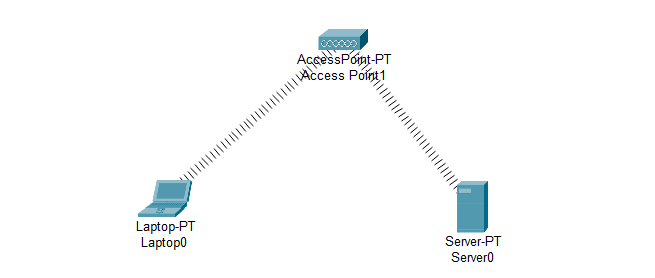
\includegraphics[keepaspectratio,alt={Capture d\textquotesingle écran de Packet Tracer : Access Point1 est en haut, Laptop0 en bas à gauche et Server0 en bas à droite. Une ligne en pointillé épais, qui représente une liaison sans fil, relie chacun des deux appareils au point d\textquotesingle accès.}]{img/wifi-connecte.png}}

}

\caption{Le serveur et l'ordinateur portable sont connectés au point
d'accès.}

\end{figure}%

Ajoutez deux autres périphériques sans fil : une tablette et un
smartphone, par exemple.

\begin{tcolorbox}[enhanced jigsaw, arc=.35mm, bottomrule=.15mm, bottomtitle=1mm, breakable, colback=white, colbacktitle=quarto-callout-note-color!10!white, colframe=quarto-callout-note-color-frame, coltitle=black, left=2mm, leftrule=.75mm, opacityback=0, opacitybacktitle=0.6, rightrule=.15mm, title=\textcolor{quarto-callout-note-color}{\faInfo}\hspace{0.5em}{Question 3}, titlerule=0mm, toprule=.15mm, toptitle=1mm]

Quelles remarques pouvez-vous faire au sujet de l'adresse IP des
terminaux ajoutés et de celle de l'ordinateur portable ? À quoi cela
est-il dû ?

\end{tcolorbox}

Passez en mode Simulation et simulez l'envoi de PDU entre ces différents
périphériques.

\begin{tcolorbox}[enhanced jigsaw, arc=.35mm, bottomrule=.15mm, bottomtitle=1mm, breakable, colback=white, colbacktitle=quarto-callout-note-color!10!white, colframe=quarto-callout-note-color-frame, coltitle=black, left=2mm, leftrule=.75mm, opacityback=0, opacitybacktitle=0.6, rightrule=.15mm, title=\textcolor{quarto-callout-note-color}{\faInfo}\hspace{0.5em}{Question 4}, titlerule=0mm, toprule=.15mm, toptitle=1mm]

Tous ces appareils communiquent-ils entre eux ?

\end{tcolorbox}

\paragraph{Consulter la page web du
serveur}\label{consulter-la-page-web-du-serveur}

\begin{enumerate}
\def\labelenumi{\arabic{enumi}.}
\tightlist
\item
  Cliquez sur la tablette, puis ouvrez l'onglet « Desktop ».
\item
  Ouvrez le navigateur (« Web Browser »).
\item
  Dans la zone URL, saisissez l'adresse IP du serveur :
  \texttt{http://192.168.0.1}, puis cliquez sur « Go ».
\end{enumerate}

La page web du serveur s'ouvre.

\begin{figure}[htbp]

{\centering \pandocbounded{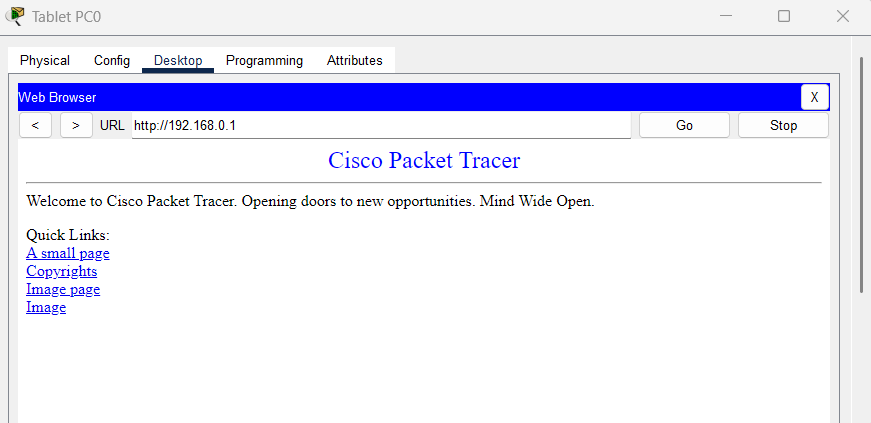
\includegraphics[keepaspectratio,alt={Capture d\textquotesingle écran de la fenêtre Tablet PC0 de Packet Tracer, onglet Desktop, navigateur Web Browser. Le champ URL contient http://192.168.0.1. La page affiche le titre Cisco Packet Tracer, la phrase Welcome to Cisco Packet Tracer. Opening doors to new opportunities. Mind Wide Open., puis quatre liens : A small page, Copyrights, Image page et Image.}]{img/tablette-page-web.png}}

}

\caption{La tablette affiche la page d'accueil du serveur.}

\end{figure}%

\subsubsection{Partie B --- Projet : trois réseaux et leurs cahiers des
charges (1
h)}\label{partie-b-projet-trois-ruxe9seaux-et-leurs-cahiers-des-charges-1-h}

Vous n'avez plus de schéma de câblage à suivre. Pour chaque réseau, un
cahier des charges fixe les contraintes, et vous choisissez le matériel
et la configuration. La figure Figure~\ref{fig-trois-reseaux} montre les
appareils de chaque réseau.

\begin{figure}[htbp]

\centering{

\pandocbounded{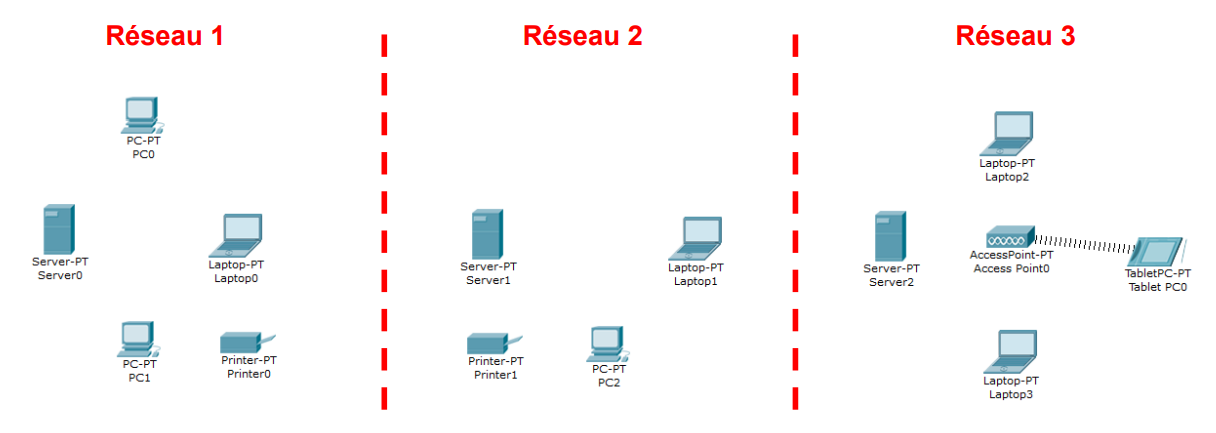
\includegraphics[keepaspectratio,alt={Capture d\textquotesingle écran de Packet Tracer, trois zones séparées par des traits verticaux rouges en pointillé. Réseau 1 : les postes PC0 et PC1, le serveur Server0, l\textquotesingle ordinateur portable Laptop0 et l\textquotesingle imprimante Printer0. Réseau 2 : le serveur Server1, l\textquotesingle ordinateur portable Laptop1, l\textquotesingle imprimante Printer1 et le poste PC2. Réseau 3 : le serveur Server2, les ordinateurs portables Laptop2 et Laptop3, un point d\textquotesingle accès Access Point0 et la tablette Tablet PC0, déjà reliée au point d\textquotesingle accès par une liaison sans fil.}]{img/trois-reseaux.png}}

}

\caption{\label{fig-trois-reseaux}Les appareils des trois réseaux à
construire.}

\end{figure}%

\begin{tcolorbox}[enhanced jigsaw, arc=.35mm, bottomrule=.15mm, bottomtitle=1mm, breakable, colback=white, colbacktitle=quarto-callout-note-color!10!white, colframe=quarto-callout-note-color-frame, coltitle=black, left=2mm, leftrule=.75mm, opacityback=0, opacitybacktitle=0.6, rightrule=.15mm, title=\textcolor{quarto-callout-note-color}{\faInfo}\hspace{0.5em}{Question 5}, titlerule=0mm, toprule=.15mm, toptitle=1mm]

Construisez puis configurez les hôtes du réseau 1 de manière à ce que la
communication soit rendue possible entre les hôtes, tout en respectant
le cahier des charges ci-dessous.

\textbf{Cahier des charges 1} : le réseau 1 est un réseau filaire avec
un adressage statique, avec le masque par défaut de la classe C
(255.255.255.0). L'ajout de concentrateur(s), de commutateur(s), de
routeur(s) et de ports est possible.

Pour les questions 9 et 10, adoptez ce plan d'adressage : le réseau 1
est 192.168.1.0/24, le poste PC0 a l'adresse 192.168.1.10 et sa
passerelle par défaut est 192.168.1.254.

\end{tcolorbox}

\begin{tcolorbox}[enhanced jigsaw, arc=.35mm, bottomrule=.15mm, bottomtitle=1mm, breakable, colback=white, colbacktitle=quarto-callout-note-color!10!white, colframe=quarto-callout-note-color-frame, coltitle=black, left=2mm, leftrule=.75mm, opacityback=0, opacitybacktitle=0.6, rightrule=.15mm, title=\textcolor{quarto-callout-note-color}{\faInfo}\hspace{0.5em}{Question 6}, titlerule=0mm, toprule=.15mm, toptitle=1mm]

Construisez puis configurez les hôtes du réseau 2 de manière à ce que la
communication soit rendue possible entre les hôtes, tout en respectant
le cahier des charges ci-dessous.

\textbf{Cahier des charges 2} : le réseau 2 est un réseau filaire avec
un adressage statique, avec le masque par défaut de la classe B
(255.255.0.0). L'ajout de concentrateur(s), de commutateur(s), de
routeur(s) et de ports est possible.

\end{tcolorbox}

\begin{tcolorbox}[enhanced jigsaw, arc=.35mm, bottomrule=.15mm, bottomtitle=1mm, breakable, colback=white, colbacktitle=quarto-callout-note-color!10!white, colframe=quarto-callout-note-color-frame, coltitle=black, left=2mm, leftrule=.75mm, opacityback=0, opacitybacktitle=0.6, rightrule=.15mm, title=\textcolor{quarto-callout-note-color}{\faInfo}\hspace{0.5em}{Question 7}, titlerule=0mm, toprule=.15mm, toptitle=1mm]

Construisez et configurez les hôtes du réseau 3 de manière à ce que la
communication soit rendue possible entre les hôtes, tout en respectant
le cahier des charges ci-dessous.

\textbf{Cahier des charges 3} : le réseau 3 est un réseau « wireless »
avec un adressage dynamique, avec le masque par défaut de la classe C
(255.255.255.0). L'ajout de concentrateur(s), de commutateur(s), de
routeur(s) et de ports est possible.

\end{tcolorbox}

\begin{tcolorbox}[enhanced jigsaw, arc=.35mm, bottomrule=.15mm, bottomtitle=1mm, breakable, colback=white, colbacktitle=quarto-callout-warning-color!10!white, colframe=quarto-callout-warning-color-frame, coltitle=black, left=2mm, leftrule=.75mm, opacityback=0, opacitybacktitle=0.6, rightrule=.15mm, title=\textcolor{quarto-callout-warning-color}{\faExclamationTriangle}\hspace{0.5em}{Attention}, titlerule=0mm, toprule=.15mm, toptitle=1mm]

Pour créer un réseau efficace et qui fonctionne bien, il est recommandé
de supprimer le point d'accès de base (AccessPoint-PT) et de le
remplacer par le point d'accès WRT300N.

Vous devez, pour la création du réseau global, utiliser un seul routeur.

\end{tcolorbox}

\begin{tcolorbox}[enhanced jigsaw, arc=.35mm, bottomrule=.15mm, bottomtitle=1mm, breakable, colback=white, colbacktitle=quarto-callout-note-color!10!white, colframe=quarto-callout-note-color-frame, coltitle=black, left=2mm, leftrule=.75mm, opacityback=0, opacitybacktitle=0.6, rightrule=.15mm, title=\textcolor{quarto-callout-note-color}{\faInfo}\hspace{0.5em}{Question 8}, titlerule=0mm, toprule=.15mm, toptitle=1mm]

Il vous faut maintenant rendre la communication possible entre les 3
réseaux, tout en respectant le cahier des charges ci-après.

\textbf{Cahier des charges final} : les réseaux 1, 2 et 3 doivent
pouvoir communiquer ensemble. Toutes les solutions matérielles et
logicielles sont possibles.

\end{tcolorbox}

\begin{tcolorbox}[enhanced jigsaw, arc=.35mm, bottomrule=.15mm, bottomtitle=1mm, breakable, colback=white, colbacktitle=quarto-callout-note-color!10!white, colframe=quarto-callout-note-color-frame, coltitle=black, left=2mm, leftrule=.75mm, opacityback=0, opacitybacktitle=0.6, rightrule=.15mm, title=\textcolor{quarto-callout-note-color}{\faInfo}\hspace{0.5em}{Question 9}, titlerule=0mm, toprule=.15mm, toptitle=1mm]

Calculez l'adresse réseau et l'adresse de diffusion (« broadcast ») du
réseau 1, avec le plan d'adressage imposé à la question 5.

\end{tcolorbox}

\begin{tcolorbox}[enhanced jigsaw, arc=.35mm, bottomrule=.15mm, bottomtitle=1mm, breakable, colback=white, colbacktitle=quarto-callout-note-color!10!white, colframe=quarto-callout-note-color-frame, coltitle=black, left=2mm, leftrule=.75mm, opacityback=0, opacitybacktitle=0.6, rightrule=.15mm, title=\textcolor{quarto-callout-note-color}{\faInfo}\hspace{0.5em}{Question 10}, titlerule=0mm, toprule=.15mm, toptitle=1mm]

La passerelle par défaut du poste PC0 (192.168.1.254) fait-elle partie
du réseau 1 ? Justifiez votre réponse.

\end{tcolorbox}

\subsection{Vérification et compte
rendu}\label{vuxe9rification-et-compte-rendu}

Votre travail est réussi si vous pouvez constater les points suivants :

\begin{itemize}
\tightlist
\item
  le serveur, l'ordinateur portable, la tablette et le smartphone sont
  connectés au point d'accès, et la page \texttt{http://192.168.0.1}
  s'affiche sur la tablette ;
\item
  chacun des trois réseaux respecte son cahier des charges (type de
  liaison, adressage statique ou dynamique, masque de la classe
  demandée) ;
\item
  les hôtes de chaque réseau communiquent entre eux ;
\item
  les hôtes des trois réseaux communiquent entre eux, avec un seul
  routeur ;
\item
  les fichiers des parties A et B sont enregistrés.
\end{itemize}

Votre compte rendu contient :

\begin{itemize}
\tightlist
\item
  les réponses aux Questions 1 à 10 ;
\item
  une capture du réseau Wi-Fi de la partie A, avec les quatre appareils
  connectés ;
\item
  une capture de la configuration du point d'accès (SSID et WPA2-PSK) ;
\item
  une capture de la page web affichée sur la tablette ;
\item
  une capture du réseau global de la partie B, avec les adresses IP
  configurées ;
\item
  une capture d'un test de communication entre deux hôtes de réseaux
  différents.
\end{itemize}

\subsection{Synthèse}\label{synthuxe8se}

\begin{tcolorbox}[enhanced jigsaw, arc=.35mm, bottomrule=.15mm, bottomtitle=1mm, breakable, colback=white, colbacktitle=quarto-callout-important-color!10!white, colframe=quarto-callout-important-color-frame, coltitle=black, left=2mm, leftrule=.75mm, opacityback=0, opacitybacktitle=0.6, rightrule=.15mm, title=\textcolor{quarto-callout-important-color}{\faExclamation}\hspace{0.5em}{Synthèse à compléter}, titlerule=0mm, toprule=.15mm, toptitle=1mm]

Recopiez et complétez ces phrases dans votre compte rendu.

\begin{enumerate}
\def\labelenumi{\arabic{enumi}.}
\tightlist
\item
  Un appareil sans fil doit être équipé d'un module
  \ldots\ldots\ldots\ldots{} pour se connecter à un point d'accès.
\item
  Pour se connecter au réseau Wi-Fi, un appareil doit connaître le
  \ldots\ldots\ldots\ldots{} du réseau et, avec WPA2-PSK, la
  \ldots\ldots\ldots\ldots{} .
\item
  Quand un appareil en DHCP ne trouve aucun serveur DHCP, il utilise une
  adresse de la plage \ldots\ldots\ldots\ldots{} (mécanisme appelé
  \ldots\ldots\ldots\ldots{} ).
\item
  Dans un réseau d'adresse 192.168.1.0/24, l'adresse réseau est
  \ldots\ldots\ldots\ldots{} et l'adresse de diffusion est
  \ldots\ldots\ldots\ldots{} .
\item
  Pour que des réseaux différents communiquent, il faut les relier avec
  un \ldots\ldots\ldots\ldots{} ; chaque hôte désigne alors son
  \ldots\ldots\ldots\ldots{} comme passerelle par défaut.
\end{enumerate}

\end{tcolorbox}

Notez enfin, en deux ou trois lignes, la difficulté principale
rencontrée pendant ce TP et la manière dont vous l'avez résolue.

\subsection{Pour aller plus loin}\label{pour-aller-plus-loin}

Votre réseau 3 est à adressage dynamique : une machine doit donc
distribuer les adresses. Dans la maquette du TP DHCP du chapitre 06, un
serveur DHCP joue ce rôle. Cherchez comment obtenir le même résultat
dans votre réseau 3, puis comparez vos solutions avec celles de vos
camarades.

Sources :

\begin{itemize}
\tightlist
\item
  RFC 3927, \emph{Dynamic Configuration of IPv4 Link-Local Addresses},
  IETF, 2005 (plage 169.254.0.0/16, adressage automatique sans serveur)
  : \url{https://www.rfc-editor.org/rfc/rfc3927}
\item
  RFC 2131, \emph{Dynamic Host Configuration Protocol}, IETF, 1997 :
  \url{https://www.rfc-editor.org/rfc/rfc2131}
\item
  Cisco, \emph{Packet Tracer}, documentation et ressources :
  \url{https://www.netacad.com/cisco-packet-tracer}
\end{itemize}




\end{document}
